\section{Results}
\label{sec:results}

Every comparison below scores the same held-out realisations with the same
metrics. Learned methods are scored only on stations the network never saw, and
each learned number is a distribution over training seeds rather than one draw.
Section~\ref{sec:results:check} shows that the harness recovers a known truth,
Sections~\ref{sec:results:t1}--\ref{sec:results:t3} give the three tasks, and
Sections~\ref{sec:results:downstream}--\ref{sec:results:external} follow the
products downstream.

\subsection{Validation of the injection and estimation pipeline}
\label{sec:results:check}

On a synthetic grid that sweeps white and flicker amplitudes, the recovered
white-noise level departs from the injected one by at most $0.0197$ in relative
terms and the flicker level shows a median relative bias of $-0.0377$. The
flicker bias is the finite-length behaviour of Whittle estimation, shared by
all methods and therefore cancelling in comparisons. For a series with known
white and flicker noise of length $n=3650$ days, the Monte-Carlo scatter of the
estimated velocity is $0.1613$~mm\,yr$^{-1}$ against a median reported GLS
uncertainty of $0.1615$~mm\,yr$^{-1}$, a calibration ratio of $1.0011$. The
estimator is calibrated to better than $0.1\%$ on the uniform grid. On the
irregularly sampled test stations the untreated series is itself below nominal
coverage (Sec.~\ref{sec:results:downstream}), so the downstream calibration is
read as a relative comparison between methods, not as an absolute statement
about geodetic uncertainty.

Figure~\ref{fig:station_noise} applies the same estimator to every benchmark
series. The recovered white and flicker levels bracket the injected 1.5 and
3.0~mm, while the recovered random walk is an upper bound because transients are
absorbed by that component.

\subsection{Task 1: denoising}
\label{sec:results:t1}

Denoising is scored as the reduction $1-\mathrm{RMSE}(\hat S,S)/\mathrm{RMSE}(y,S)$
on the same realisations, where $y$ is the noisy series and $S$ the truth.
Figure~\ref{fig:truth_families} shows the construction of the two families and
the per-station scores.

\begin{figure}[t]
\centering
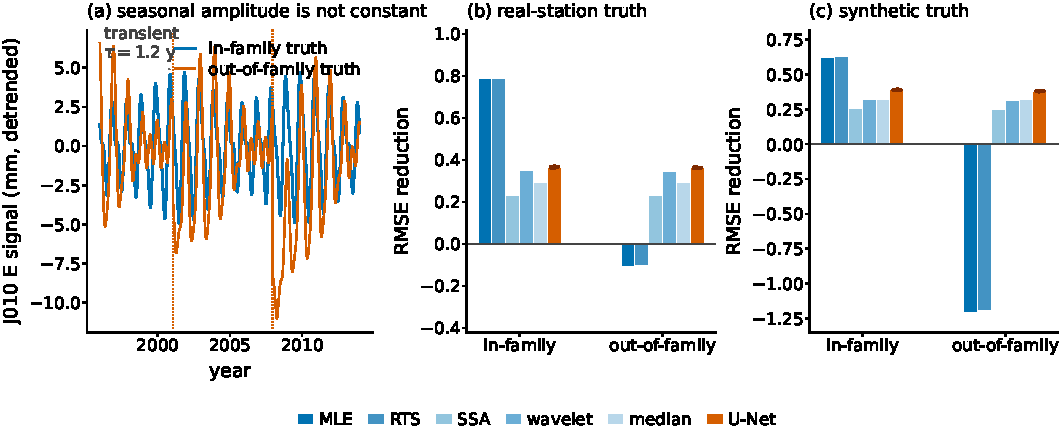
\includegraphics[width=\linewidth]{figures/fig08_truth_families.pdf}
\caption{Parametric denoising depends on the truth family; the learned one does
not. (a) The out-of-family truth modulates the annual amplitude, adds exponential
transients (dotted epochs) and a logarithmic relaxation; the in-family truth
keeps the amplitude nearly constant. (b) On real-station truth the trajectory
model and RTS smoother dominate in-family and fall below zero out-of-family,
whereas the U-Net stays between $0.363$ and $0.366$ and sits above every
model-free decomposition in both families. (c) The fully synthetic grid shows the same
pattern. Bars are means over realisations, orange dots are individual training
seeds, and classical methods are deterministic.}
\label{fig:truth_families}
\end{figure}

On the in-family truth, where the signal is the trend--harmonic trajectory fitted
to a real station, the parametric estimator reproduces its earlier result: the
trajectory model reduces the error by $0.790$ (95\% bootstrap interval
$0.776$--$0.804$) and the Kalman/RTS smoother by $0.791$. The model-free
decompositions follow at a distance: wavelet $0.349$, moving median $0.293$, SSA
$0.232$. The U-Net, scored with the per-window normalisation used in training,
reaches $0.366 \pm 0.002$ over ten seeds. It does not reach the parametric
estimators, which see the correct basis, but it is above every model-free
decomposition in the same regime.

The out-of-family truth keeps the same stations but adds a multiplicative
seasonal modulation, exponential transients and logarithmic post-seismic
relaxation. The trajectory model falls to $-0.106$ (interval $-0.434$ to
$0.181$) and the RTS smoother to $-0.104$: with this truth the fit can leave the
series noisier than it found it. The model-free methods barely move (wavelet
$0.345$, median $0.292$, SSA $0.231$), because none of them assumes a stationary
harmonic basis. The U-Net, trained on the out-of-family generator, is almost
unchanged at $0.363 \pm 0.001$ and is now the strongest method apart from the
untreated series.

The fully synthetic regimes make the same point with more realisations.
In-family, the trajectory model reduces the error by $0.624$ and the U-Net by
$0.389 \pm 0.001$; the moving median reaches $0.320$, the wavelet $0.317$ and
SSA $0.252$. Out-of-family, the trajectory model drops to $-1.211$ while the
U-Net stays at $0.381 \pm 0.001$, against $0.318$ for the median and $0.312$ for
the wavelet. The learned denoiser therefore overtakes the model-free
decompositions in all four regimes, on both the real-station and the fully
synthetic truth, and its score changes by less than $0.01$ when the truth family
changes. The denoising conclusion is conditional only on the parametric
alternative: the trajectory model wins by more than a factor of two when the
truth lies in its basis and adds error when it does not, while the learned
denoiser is the best non-parametric choice in both families.

The difference from the first version comes from the inference protocol, not
from the truth construction. Scoring the same networks on whole-series
normalisation returns $0.193$ in-family and $0.274$ out-of-family, which is why
the earlier draft placed the U-Net below SSA on real stations. Matching the
normalisation to the training windows removes that gap and leaves the ordering
above.

\subsection{Task 2: gap filling}
\label{sec:results:t2}

Gap filling is scored on 40 held-out component series of long synthetic records
and on 30 held-out component series of real stations, with gaps of 5, 30 and 120
days. Two inference modes are reported for the network: whole-series
normalisation, the protocol of the first version, and per-window normalisation,
which matches the statistics under which the network was trained.

On long synthetic records (Table~\ref{tab:t2}), the 5-day gap is filled best by
SSA ($2.57$~mm), followed by linear interpolation ($2.69$) and the per-window
U-Net ($2.80 \pm 0.06$); the trajectory model is at $3.41$. At 30 days the order
changes: the per-window U-Net reaches $3.07 \pm 0.03$ and beats linear
interpolation ($3.34$), SSA ($3.37$), PCHIP ($3.59$) and the trajectory model
($3.79$). At 120 days the trajectory model is best ($3.99$), the per-window
U-Net reaches $5.09 \pm 0.08$, and whole-series inference fails at
$7.59 \pm 0.26$.

\begin{table}[t]
\centering
\caption{Gap-filling error (RMSE at the missing days, mm) for long synthetic
series ($n=40$ component series) and real held-out stations ($n=30$). The
per-window U-Net is the best method at 30-day gaps on both record sets, but the
real-set margin does not survive the full 201 component series
(Sec.~\ref{sec:results:external}); the trajectory model is best at 120 days,
and the whole-series arm fails. Values for
the network are means over ten training seeds with the seed standard deviation.}
\label{tab:t2}
\setlength{\tabcolsep}{3pt}
\begin{tabular}{lccccc}
\hline
 & \multicolumn{3}{c}{Long synthetic} & \multicolumn{2}{c}{Real stations} \\
\cmidrule(lr){2-4}\cmidrule(lr){5-6}
Method & 5~d & 30~d & 120~d & 5~d & 30~d \\
\hline
Linear         & 2.69 & 3.34 & 4.72 & 2.65 & 2.93 \\
PCHIP          & 2.80 & 3.59 & 5.22 & 2.76 & 3.10 \\
SSA            & 2.57 & 3.37 & 4.73 & 2.51 & 2.97 \\
Trajectory MLE & 3.41 & 3.79 & 3.99 & 3.16 & 3.35 \\
\hline
U-Net, whole series & $4.52 \pm 0.54$ & $3.55 \pm 0.14$ & $7.59 \pm 0.26$ & $9.98 \pm 1.80$ & $6.16 \pm 0.60$ \\
U-Net, per window   & $2.80 \pm 0.06$ & $3.07 \pm 0.03$ & $5.09 \pm 0.08$ & $2.55 \pm 0.03$ & $2.74 \pm 0.03$ \\
\hline
\end{tabular}
\end{table}

The real stations reproduce the same pattern (Table~\ref{tab:t2}). At 5 days SSA
($2.51$~mm) and the per-window U-Net ($2.55 \pm 0.03$) are tied, with linear
interpolation at $2.65$; at 30 days the per-window U-Net leads at
$2.74 \pm 0.03$ against $2.93$ for linear interpolation and $2.97$ for SSA. The
whole-series arm is not competitive at either length ($9.98 \pm 1.80$ and
$6.16 \pm 0.60$), up to a factor of four worse than the same network evaluated
per window. The gap-filling failure reported in the first version was therefore
an inference-normalisation defect, not an inability of the architecture to
interpolate. With the defect removed, the learned imputer leads at 30-day gaps
on synthetic records and on this 30-series real subset, but not across the full
held-out set (Sec.~\ref{sec:results:external}); it loses at 5 days by a small
margin and at 120 days by a large one. Fig.~\ref{fig:impute_log} shows the same scores on a log
scale, with seed error bars. The per-window curve rises by at most $0.3$~mm
between 5 and 30 days, while the whole-series arm is $1.7$~mm above it at 5 days
on the synthetic records and $7.4$~mm above it on the real stations.

\begin{figure}[t]
\centering
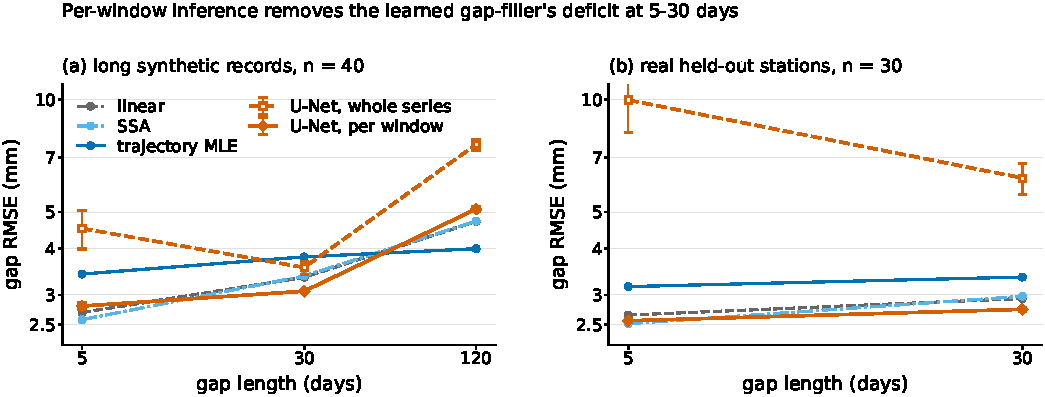
\includegraphics[width=\linewidth]{figures/fig06_impute_log.pdf}
\caption{Gap-filling error against gap length. Per-window inference (solid
orange, diamonds) is within 0.1~mm of SSA at 5 days and best at 30 days on both
long synthetic records (a) and real held-out stations (b); the trajectory model
remains best at 120 days. The whole-series arm (dashed, open squares) is not a
competitive configuration at any length. Error bars are one standard deviation
over ten training seeds; classical methods are deterministic and carry none.}
\label{fig:impute_log}
\end{figure}

The trajectory model's advantage at long gaps is visible in signal error rather
than observation error: against the missing true signal, its RMSE is $0.74$~mm
at 5 days, $0.68$ at 30, $0.78$ at 120 and $0.78$ at 365 days, while the
whole-series network reaches $11.40$, $5.97$, $10.26$ and $61.0$~mm at the same
lengths. That arm is the defective configuration, and we do not extrapolate the
30-day per-window win to year-long gaps, for which no per-window measurement was
made.

\subsection{Task 3: offset detection under a fair protocol}
\label{sec:results:t3}

Both detectors are reduced to a decision field, a threshold and a minimum
separation, so the comparison measures the field rather than a tuning accident.
Offsets of 2, 4, 8, 16 and 25~mm are injected at known epochs; a detection within
30 days counts as a match, and two accepted detections must be at least 45 days
apart. The threshold is selected per seed on held-out validation draws, which is
the protocol a user would follow, and we also report the oracle threshold.

At the validation-selected threshold the classical detector has the higher F1 at
every amplitude (Table~\ref{tab:t3}): $0.073$ against $0.0005$ at 2~mm, $0.259$
against $0.039$ at 4~mm, $0.815$ against $0.460$ at 8~mm, $0.963$ against
$0.709$ at 16~mm and $0.975$ against $0.725$ at 25~mm
(Fig.~\ref{fig:fair_detector}). The learned field nevertheless ranks large
steps better: its average precision is higher at 16~mm ($0.648$ against $0.208$)
and at 25~mm ($0.669$ against $0.007$). The two metrics answer different
questions. Average precision integrates over all thresholds and rewards a field
that orders events well; the deployed detector uses one threshold, and there the
classical field is better. Reporting only average precision would have hidden
that its operating point is worse.

\begin{figure}[t]
\centering
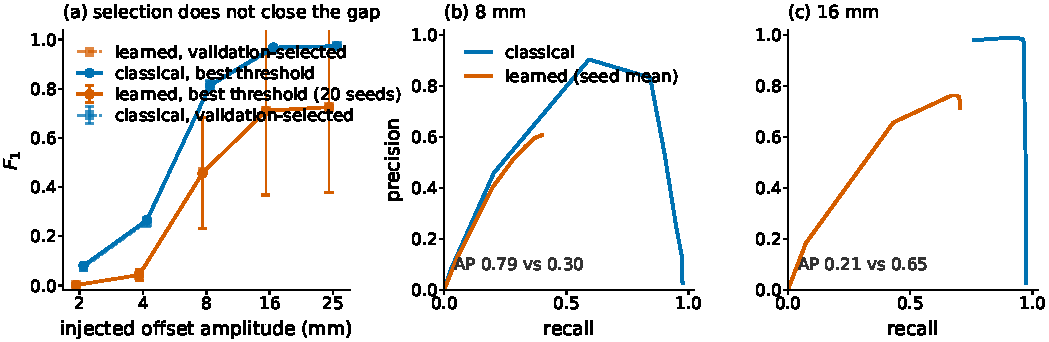
\includegraphics[width=\linewidth]{figures/fig13_fair_detector.pdf}
\caption{Threshold selection does not close the detection gap. (a) Validation-
selected and oracle $F_1$ for the classical and learned fields: the learned
field improves when its threshold is tuned, but not enough to meet the classical
detector at any amplitude. (b),(c) Precision--recall curves at 8 and 16~mm: the
learned field has lower average precision at 8~mm and higher at 16~mm, which is
the ranking-versus-operating-point distinction in the text. The learned seed mean
is shown with one standard deviation; classical detection is deterministic.}
\label{fig:fair_detector}
\end{figure}

\begin{table}[t]
\centering
\caption{Synthetic offset detection by injected amplitude. The threshold is
selected on held-out validation draws for every seed. The learned field has
higher average precision at 16 and 25~mm, but at the operating point a user
would deploy its F1 is lower at every amplitude. Learned values are means over
twenty seeds; the F1 column also gives the seed standard deviation.}
\label{tab:t3}
\footnotesize
\setlength{\tabcolsep}{4pt}
\begin{tabular}{ccccc}
\hline
Amplitude (mm) & Classical AP & Classical F1 & Learned AP & Learned F1 \\
\hline
2  & 0.032 & 0.073 & 0.0000 & $0.0005 \pm 0.002$ \\
4  & 0.143 & 0.259 & 0.0028 & $0.0395 \pm 0.024$ \\
8  & 0.788 & 0.815 & 0.298  & $0.460 \pm 0.222$ \\
16 & 0.208 & 0.963 & 0.648  & $0.709 \pm 0.334$ \\
25 & 0.007 & 0.975 & 0.669  & $0.725 \pm 0.341$ \\
\hline
\end{tabular}
\end{table}

\subsection{Task 3 on real catalogue labels}
\label{sec:results:t3:real}

The NGL discontinuity catalogue supplies 1\,743 labels on 153 held-out component
series from 58 stations: 52 code-1 and 1\,691 code-2 entries, distributed over
1006 East, 528 North and 209 Up series. The labels are matched to the series,
restricted to the record span and to offsets whose observed amplitude exceeds
three times the local noise level, and deduplicated at 60 days. Amplitudes are
skewed (median $-6.23$~mm, interquartile range $-17.79$ to $11.61$~mm) and
concentrated in East, which is where the catalogue is densest. Stations, not
series, are split into validation and scoring halves over 40 draws, so a
detector never chooses a threshold on the stations it is scored on.

The classical detector reaches F1 $0.457 \pm 0.027$, average precision $0.322$,
precision $0.490$ and recall $0.536$. Recall rises with signal-to-noise ratio,
from $0.398$ in the 3--5 stratum to $0.610$ in 5--10 and $0.848$ above 10.
Its median signed delay is $-51.5$ days, with an absolute median of $69.7$ days.
The twenty U-Net seeds average F1 $0.232 \pm 0.107$ and average precision
$0.135$; precision is $0.329$ and recall $0.302$. Three seeds collapse to
essentially no detections (F1 $0.0000$, $0.0002$ and $0.0004$), which is why the
seed mean is far below the median seed ($0.290$). The best seed reaches $0.316$.
The ten TCN seeds average F1 $0.273 \pm 0.096$, average precision $0.173$,
precision $0.368$ and recall $0.356$, with one collapsed seed and a best seed of
$0.319$. The TCN is therefore the stronger of the two learned architectures on
every aggregate metric, and it is still the weaker detector: even its best seed
lies below the classical mean minus one standard deviation ($0.430$). Where a
U-Net seed does detect events, its absolute median delay is $16.5$--$52.1$ days
and its signed median lies between $-18.3$ and $+1.0$ days; the TCN range is
$7.8$--$39.9$ days, signed between $-4.8$ and $+0.7$ days. Matched learned
detections sit closer to the catalogued epoch than the classical ones, while the
classical detector finds more of them at lower precision.

Real labels are harder than synthetic ones for both detectors. The classical F1
falls from $0.815$ at 8~mm in the synthetic protocol to $0.457$ on the catalogue,
and the U-Net F1 from $0.460$ to $0.232$. The same classical advantage holds for
the TCN on the synthetic subset scored in Sec.~\ref{sec:results:arch}. Neither
learned architecture changes the ordering.
The regional split shows the same shortfall everywhere the catalogue is dense:
Asia, which supplies 39 of the 58 labelled stations, gives the classical
detector F1 $0.488$, the U-Net $0.251$ and the TCN $0.294$; North America gives
$0.426$, $0.230$ and $0.272$. Europe is the weakest region for every method
($0.267$, $0.101$ and $0.109$) and has only six labelled stations, so its
ranking is the least stable. The centre and region ordering is shared by the
classical and learned arms, which rules out a single-region artefact as the
explanation of the learned shortfall. Figure~\ref{fig:real_offsets} shows the
per-seed distribution, the signal-to-noise strata and the delay.

\begin{figure}[t]
\centering
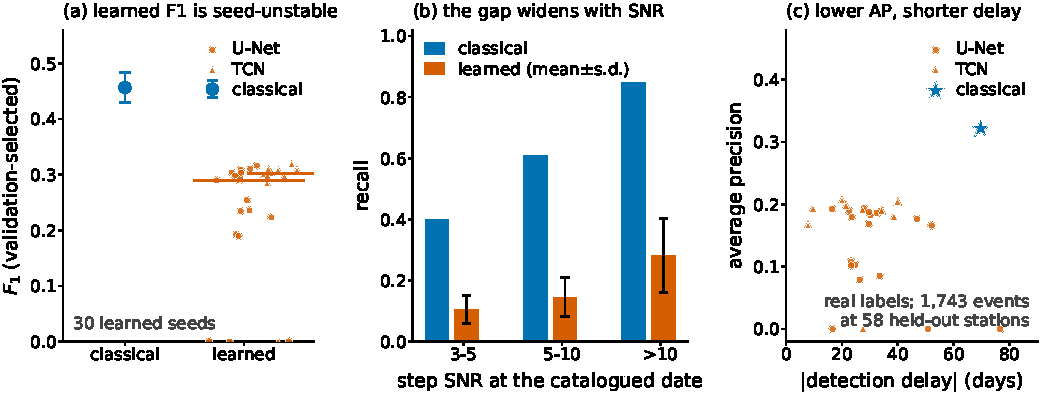
\includegraphics[width=\linewidth]{figures/fig09_real_offsets.pdf}
\caption{Detection against 1\,743 real catalogue labels. (a) The twenty U-Net
and ten TCN seeds spread from near-zero to just above the classical $F_1$, and
four seeds collapse; both learned means stay below the classical mean, and the
TCN mean is the higher of the two. (b) Recall rises with signal-to-noise ratio
for the classical detector, while the learned mean stays lower in every stratum.
(c) The learned fields have lower average precision but shorter matched delays;
they find fewer events, and the ones they find sit closer to the catalogued
epoch. Bars and points are seed statistics; the classical detector is
deterministic.}
\label{fig:real_offsets}
\end{figure}

\subsection{Downstream velocity and the random-walk arm}
\label{sec:results:downstream}

A benchmark product is only useful if the processed series yields a defensible
velocity. We therefore carry every method through the same GLS velocity fit on
six held-out stations and two components with three injected realisations each
(36 station--component--realisation draws per arm). Two noise models are used:
white plus flicker noise, and the same model with a random-walk component at
$\sigma_{\rm RW}=1.0$~mm\,yr$^{-1/2}$.

With white plus flicker noise, the trajectory MLE on the raw series has velocity
bias $-0.0024$~mm\,yr$^{-1}$ and RMSE $0.0586$~mm\,yr$^{-1}$. The classical
denoisers leave this essentially unchanged on the raw-noise arm: SSA $0.0588$,
RTS $0.0594$, moving median $0.0590$ and wavelet $0.0616$. The U-Net denoiser,
scored with training-matched per-window normalisation, reaches
$0.0605$~mm\,yr$^{-1}$ and a bias of $-0.0034$; its two seeds score
$0.0600$ and $0.0611$. At 30-day gaps the classical imputers are indistinguishable from the
complete series ($0.0581$--$0.0588$), and the U-Net imputer matches them at
$0.0586$. No method improves the velocity over the untreated series, but the
learned denoiser is no longer an outlier: it sits between the moving median and
the wavelet, $0.002$~mm\,yr$^{-1}$ behind the raw series.

That difference from the first version matters. Under whole-series
normalisation the same network produced $0.2087$~mm\,yr$^{-1}$; scoring it
window by window removes the mismatch and brings the velocity error back to the
level of the classical denoisers. The earlier negative downstream result was
therefore an inference-protocol artefact, not a property of learned denoising.

Calibration is quoted with the noise model estimated on the raw series and held
fixed for every method, because re-estimating the noise on a denoised output is
not a valid protocol: the trajectory and RTS outputs retain essentially no
residual, so a Whittle fit to them returns a near-zero noise level and a
vanishing reported uncertainty (calibration ratios $1.7\times10^{-14}$ and
$1.0\times10^{-6}$ in that arm). Against the raw-series noise model, the
reference reports a median velocity uncertainty of $0.0380$~mm\,yr$^{-1}$
against an empirical scatter of $0.0585$, a calibration ratio of $0.649$ and
1$\sigma$ coverage of $0.389$; classical denoisers stay between $0.618$ and
$0.647$, and the U-Net reaches $0.628$ with coverage $0.458$. The
under-coverage is the same irregular-sampling effect noted in
Sec.~\ref{sec:results:check}, which is why the ratios are comparable across
methods but should not be read as absolute geodetic uncertainties.

\begin{sloppypar}
Adding the random-walk component degrades the reference modestly and changes no
ordering. The raw/MLE bias moves from $-0.0024$ to $-0.0089$~mm\,yr$^{-1}$,
the RMSE from $0.0586$ to $0.0690$, the calibration ratio from $0.649$ to
$0.575$ and the 1$\sigma$ coverage stays at $0.389$. The classical denoisers
move to $0.0686$--$0.0713$; the U-Net denoiser reaches $0.0698$ with
calibration $0.570$ and coverage $0.403$, and the U-Net imputer $0.0690$ with
calibration $0.575$ and coverage $0.417$. The learned arms again track the
reference and the classical denoisers.
\end{sloppypar}
Fig.~\ref{fig:calibration} collects the calibration and coverage pairs, and
Fig.~\ref{fig:rw_effect} isolates the random-walk increment. The downstream
evidence is neutral: under the protocol-matched inference, neither learned arm
improves the velocity or its uncertainty, and neither destroys them.

\begin{figure}[t]
\centering
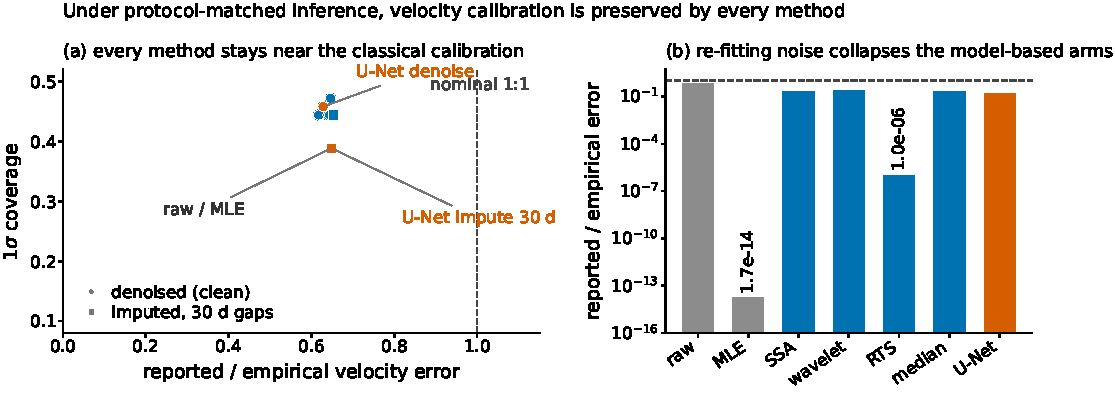
\includegraphics[width=\linewidth]{figures/fig07_calibration.pdf}
\caption{Protocol-matched inference keeps velocity calibration for every
method. (a) Reported uncertainty against empirical scatter for the clean arm:
the untreated series, the classical denoisers and both learned arms sit between
$0.62$ and $0.65$ with $1\sigma$ coverage of $0.39$--$0.47$; the learned
denoiser reaches $0.628$ and $0.458$. (b) Re-estimating the noise on each
output collapses the reported uncertainty for the trajectory MLE and the RTS
smoother ($1.7\times10^{-14}$ and $1.0\times10^{-6}$), because their residual is
nearly empty; the remaining methods stay within a factor of five of nominal.
That collapse is an artefact of the protocol, not a property of the method. The
vertical distance to the nominal line is the calibration error.}
\label{fig:calibration}
\end{figure}

\begin{figure}[t]
\centering
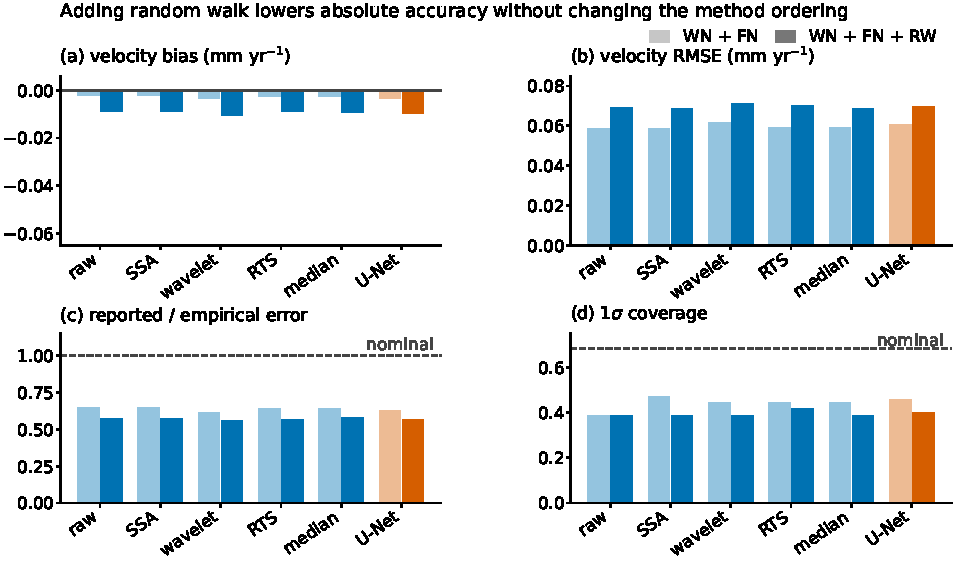
\includegraphics[width=\linewidth]{figures/fig12_rw_effect.pdf}
\caption{Adding a random-walk component changes the level, not the ordering.
Paired bars compare the white-plus-flicker arm (pale) with the white-plus-
flicker-plus-random-walk arm (solid) for velocity bias, velocity RMSE,
calibration ratio and $1\sigma$ coverage. Every method loses absolute accuracy
under the random-walk model (RMSE rises by about $0.010$~mm\,yr$^{-1}$) and
calibration falls from about $0.65$ to $0.57$; the ordering is unchanged and the
learned arms track the classical ones. Horizontal lines mark zero bias, the
nominal calibration ratio of one and the nominal $1\sigma$ coverage of $0.683$.}
\label{fig:rw_effect}
\end{figure}

\subsection{External and regional validation}
\label{sec:results:external}

The scores above come from the ten-station real subset and the thirty-series
long-record subset. To check whether they are a property of the benchmark or of
those subsets, we score every held-out test series under the same per-window
protocol: 67 series, 201 component series, of which 183 are NGL and 18 JPL,
split into Europe (18), North America (30), Asia (123), Pacific (24) and other
(6). Each component series receives three injected realisations and the ten
denoising and ten gap-filling checkpoints. No network is retrained and no
threshold is chosen, so the arm is descriptive: it asks whether the ranking
transfers, not whether a JPL-trained network would do better.

Denoising transfers. The U-Net removes $0.360 \pm 0.003$ on NGL and
$0.345 \pm 0.005$ on JPL, against $0.341$ and $0.317$ for the wavelet, $0.291$
and $0.322$ for the moving median and $0.230$ and $0.254$ for SSA. The
trajectory MLE stays ahead at $0.775$ and $0.665$. The learned denoiser is above
every model-free decomposition in both centres, and across the five regions its
mean lies between $0.333$ and $0.366$, against $0.700$--$0.812$ for the MLE and
$0.299$--$0.360$ for the wavelet. The one exception is Europe, where the U-Net
($0.358$) and the wavelet ($0.360$) are within $0.002$ of each other. The
denoising conclusion of Sec.~\ref{sec:results:t1} therefore does not depend on
the subset used to measure it.

Gap filling does not transfer as cleanly. On NGL the U-Net reaches
$2.964 \pm 0.034$~mm and linear interpolation $2.967$ [2.914, 3.017], with SSA at
$3.000$ and the MLE at $3.252$: a tie. On JPL the U-Net reaches
$3.293 \pm 0.042$ against $3.233$ [3.056, 3.416] for linear interpolation, with
SSA at $3.309$ and the MLE at $3.367$: the learned arm is $0.06$~mm behind. The
$2.74$~mm score of Sec.~\ref{sec:results:t2} came from a 30-series real subset;
on the full 201 component series the 30-day advantage is a tie on the NGL
majority and is absent on JPL. The regional split repeats the pattern: the U-Net
is the best filler in Asia ($2.990$ against $2.994$) and Europe ($2.910$ against
$3.028$), but linear interpolation is better in North America ($2.942$ against
$2.954$), the Pacific ($2.986$ against $3.089$) and the residual group ($3.068$
against $3.113$). The differences are at most $0.12$~mm, and
they do not support a product-level claim for learned gap filling on real data.
Fig.~\ref{fig:external} shows both tasks by centre and by region.

\begin{figure}[t]
\centering
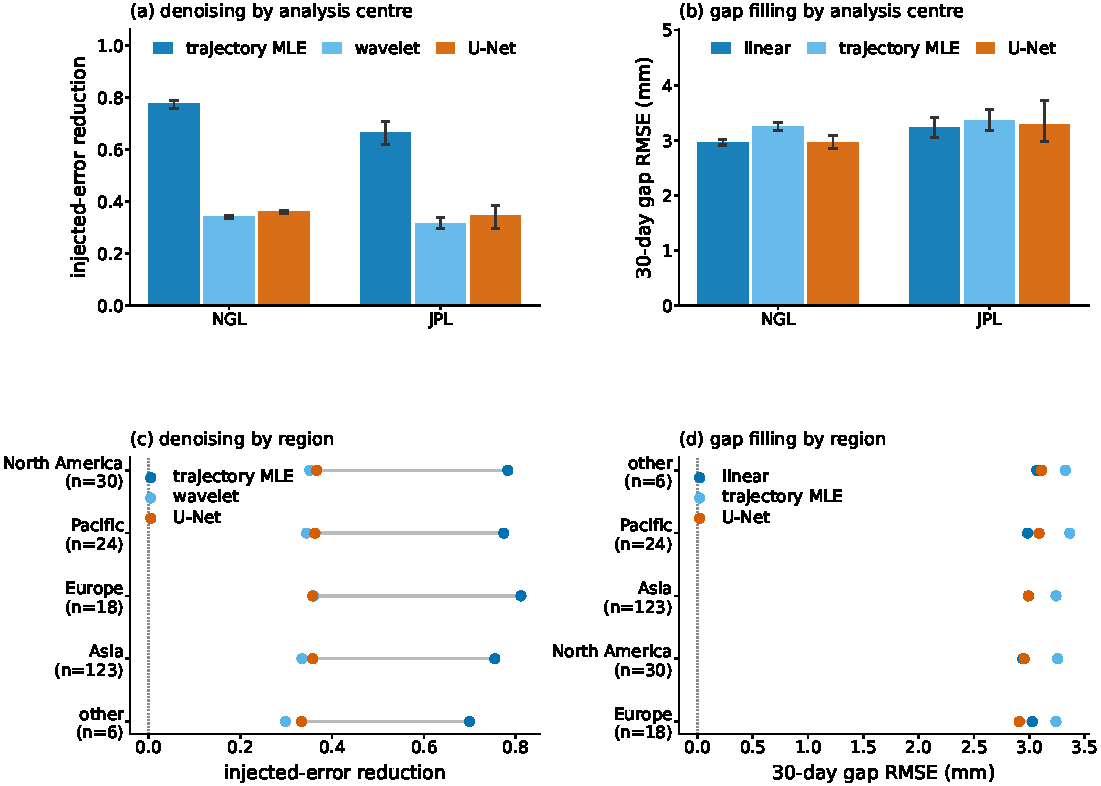
\includegraphics[width=\linewidth]{figures/fig15_external_regional.pdf}
\caption{The denoising ranking transfers across centres and regions; the
30-day gap-filling advantage does not. (a) Denoising and (b) 30-day gap filling
by analysis centre (NGL, JPL). (c)--(d) The same scores by region. Bars and
points are means over component series, with 95\% bootstrap intervals over
series for the classical methods; the learned value is the mean over ten
checkpoints and its seed standard deviation is smaller than the marker. The
learned denoiser stays above every model-free decomposition at both centres,
while the learned imputer ties linear interpolation on NGL and falls behind it
on JPL.}
\label{fig:external}
\end{figure}

\subsection{Architecture and seed variation}
\label{sec:results:arch}

The ranking is not a property of one architecture. Three learned families are
scored on the shared test split under one protocol: the U-Net (ten seeds for
denoising and gap filling, twenty for detection), the TCN (ten seeds per task)
and the smaller BiGRU of the first version (four seeds for denoising and gap
filling). Denoising and gap filling use ten held-out stations; detection uses
eight stations with one realisation, so its absolute levels are not comparable
with the twelve-station table above, only the architecture ordering within the
arm is.

Denoising is nearly architecture-independent. The U-Net reaches $0.364 \pm
0.001$, the TCN $0.365 \pm 0.001$ and the BiGRU $0.381 \pm 0.004$, all far
below the trajectory MLE at $0.815$ and above the wavelet ($0.351$), the moving
median ($0.292$) and SSA ($0.232$). The gap between the two convolutional
designs is $0.001$, inside the seed spread of either.

Gap filling separates the architectures more. At 30 days the BiGRU reaches
$2.892 \pm 0.051$~mm, the TCN $2.979 \pm 0.055$ and the U-Net $3.079 \pm
0.069$; linear interpolation is at $3.130$, SSA at $3.111$ and the trajectory
model at $3.237$. The order is the same at 5 days ($2.378 \pm 0.007$,
$2.401 \pm 0.016$ and $2.537 \pm 0.065$, against $2.508$ for linear and
$2.540$ for SSA). At 120 days the trajectory model wins at $3.230$ and the
learned arms reach $3.577 \pm 0.039$, $3.700 \pm 0.037$ and $3.705 \pm 0.045$,
with linear interpolation at $3.650$. The recurrent arm is the best learned
imputer and costs $5.1$~h per seed, against $8$~min for the U-Net and
$6$~min for the TCN; its advantage over the TCN is $0.09$~mm, which is a poor
return on a roughly fifty-fold training cost.

Detection is where architecture matters. At 8~mm the classical detector reaches
$0.761$; the TCN averages $0.568 \pm 0.207$ over ten seeds (median $0.637$) and
the U-Net $0.436 \pm 0.222$ over twenty (median $0.554$). At 16~mm the three
values are $0.947$, $0.829$ and $0.686$, and at 25~mm $0.927$, $0.791$ and
$0.675$. The TCN is ahead of the U-Net at every amplitude, and neither learned
arm reaches the classical operating point above 4~mm. At 2 and 4~mm the learned
fields are close to silent (at most $0.011$) while the classical detector scores
$0.058$ and $0.260$. The seed distribution, not the architecture, is the
dominant term: at 8~mm three U-Net seeds and one TCN seed detect nothing, and
the mean consequently sits well below the median. A single-seed comparison
would have described either architecture as a success or a failure according to
the draw. The real-label ranking agrees: TCN $0.273$ over U-Net $0.232$, both
below the classical $0.457$. Fig.~\ref{fig:architecture_seed} shows the three
seed distributions side by side.

\begin{figure}[t]
\centering
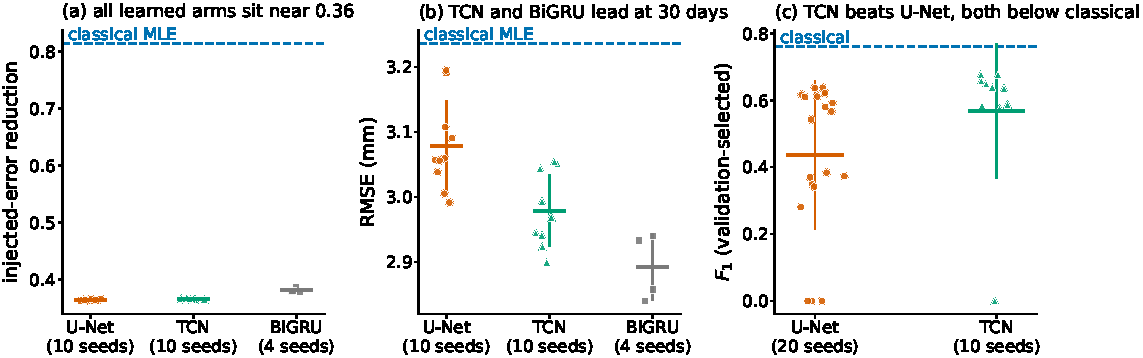
\includegraphics[width=\linewidth]{figures/fig10_architecture_seed.pdf}
\caption{Three architectures under one protocol. (a) Denoising error reduction
for the U-Net, TCN and BiGRU: the three means lie within $0.02$ of one another
and far below the trajectory MLE (dashed). (b) 30-day gap RMSE: TCN and BiGRU
are closer to the classical MLE than the U-Net, and all three beat linear
interpolation. (c) Detection at 8~mm: the TCN is ahead of the U-Net, and both
are below the classical detector (dashed). Dots are training seeds, horizontal
bars are means and vertical bars are $\pm$1~s.d.; the spread, not the mean
difference, dominates panel (c).}
\label{fig:architecture_seed}
\end{figure}
